\documentclass{article}
\usepackage{geometry}
\usepackage{graphicx}

\title{Mosquito Surveillance}
\author{Florida Department of Health - Alachua County}
\usepackage{Sweave}
\begin{document}
\Sconcordance{concordance:mosq04nov13.tex:mosq04nov13.Rnw:%
1 3 1 1 20 2 1 1 0 6 1 1 66 1 3 15 1 1 15 1 3 2 1 1 25 1 2 21 1 1 44 1 %
3 9 1 1 104 1 3 11 1 1 81 1 2 14 1 1 74 1 4 8 1 1 73 1 3 9 1 1 72 1 3 8 %
1 1 72 1 3 8 1 1 72 1 3 8 1 1 72 1 2 2 1}

\maketitle
\begin{center}
Joe Brew\\
Joseph.Brew@FLHealth.gov\\

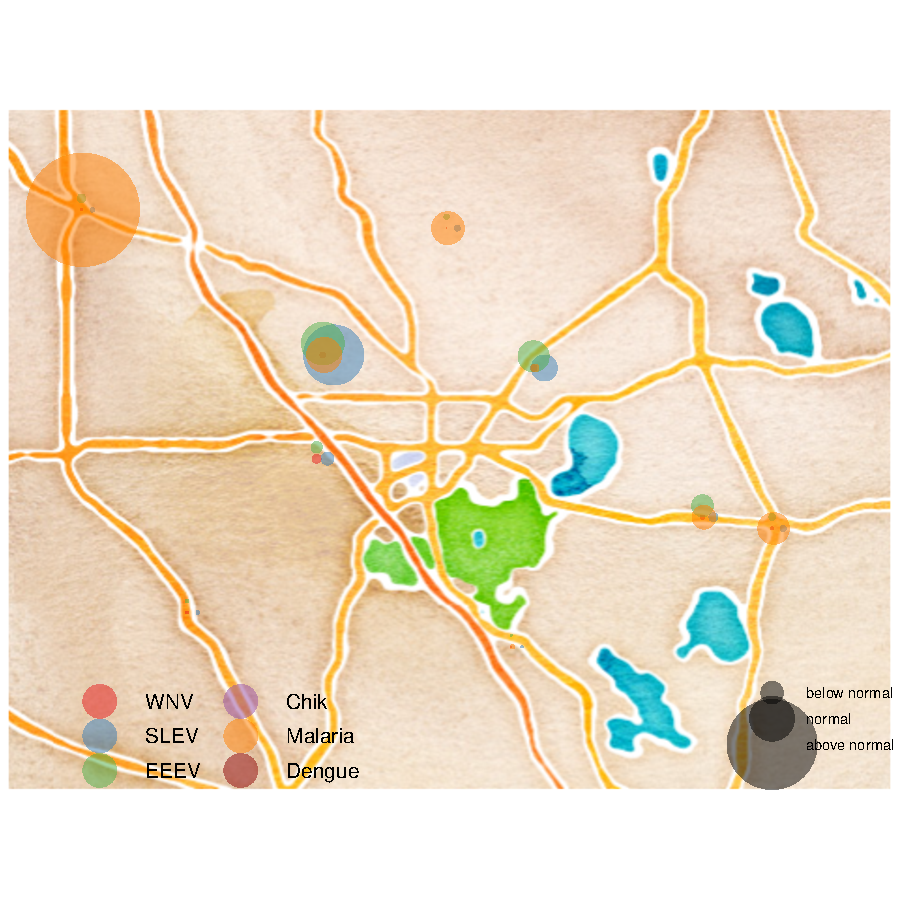
\includegraphics{mosq04nov13-002}
\end{center}
\newpage
\tableofcontents


\newgeometry{margin=1.5cm}


\begin{center}
\section*{Overview}
\addcontentsline{toc}{section}{Overview}

\end{center}
The number of mosquitoes capable of carrying disease (vectors) caught in local traps over the last four weeks remains low.

\begin{center}
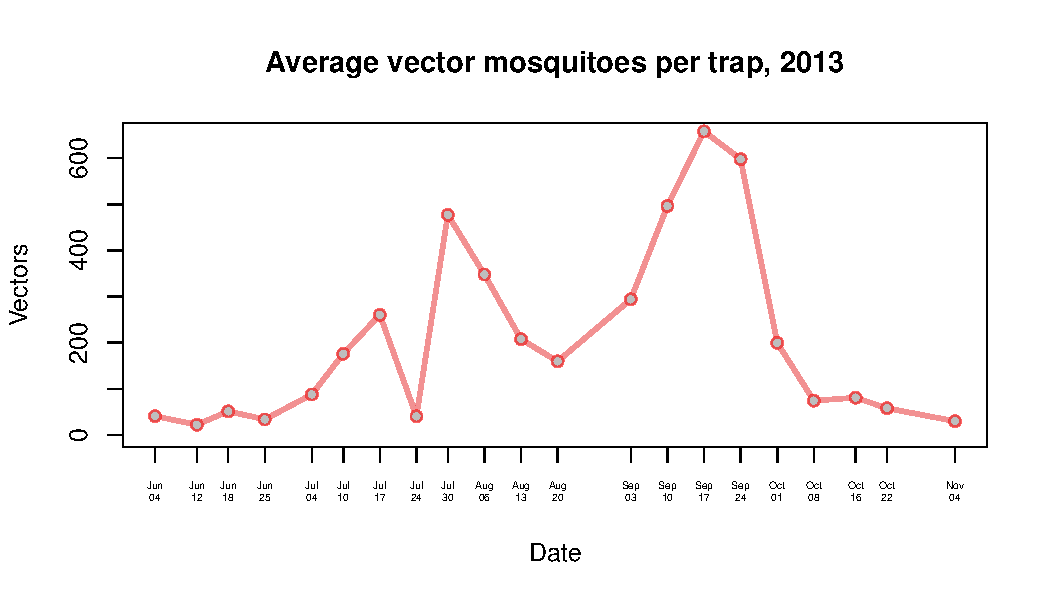
\includegraphics{mosq04nov13-003}
\end{center}
By historical standards, we are at normal (low) levels for this time of year.
\begin{center}
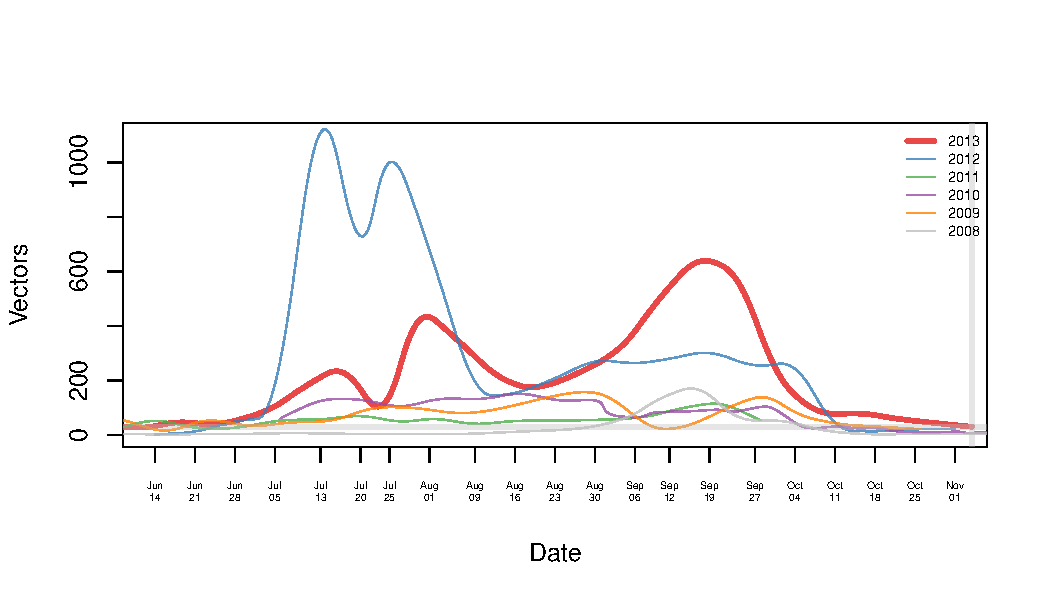
\includegraphics{mosq04nov13-004}
\end{center}
\subsection*{Recommendation}
\addcontentsline{toc}{section}{RECOMMENDATION}

No action called for at this time.
\newpage
\begin{center}
\section*{Disease Type Overview}
\addcontentsline{toc}{section}{Disease Type Overview}

\end{center}
The populations of 6 vector types are monitored specifically for the diseases which they are capable of carrying.  These disease types are:\\
\begin{enumerate}
  \item WNV (West Nile Virus)
  \item SLEV (St. Louis Encephalitis Virus)
  \item EEEV (Eastern Equine Encephalitis Virus)
  \item Chkungunya
  \item Malaria
  \item Dengue\\
\end{enumerate}
Of these vector types, 5 of the 6 declined or remained steady in the two most recent trappings.  Only Malaria vectors saw an increase (albeit very slight relative to earlier this summer).
\begin{center}
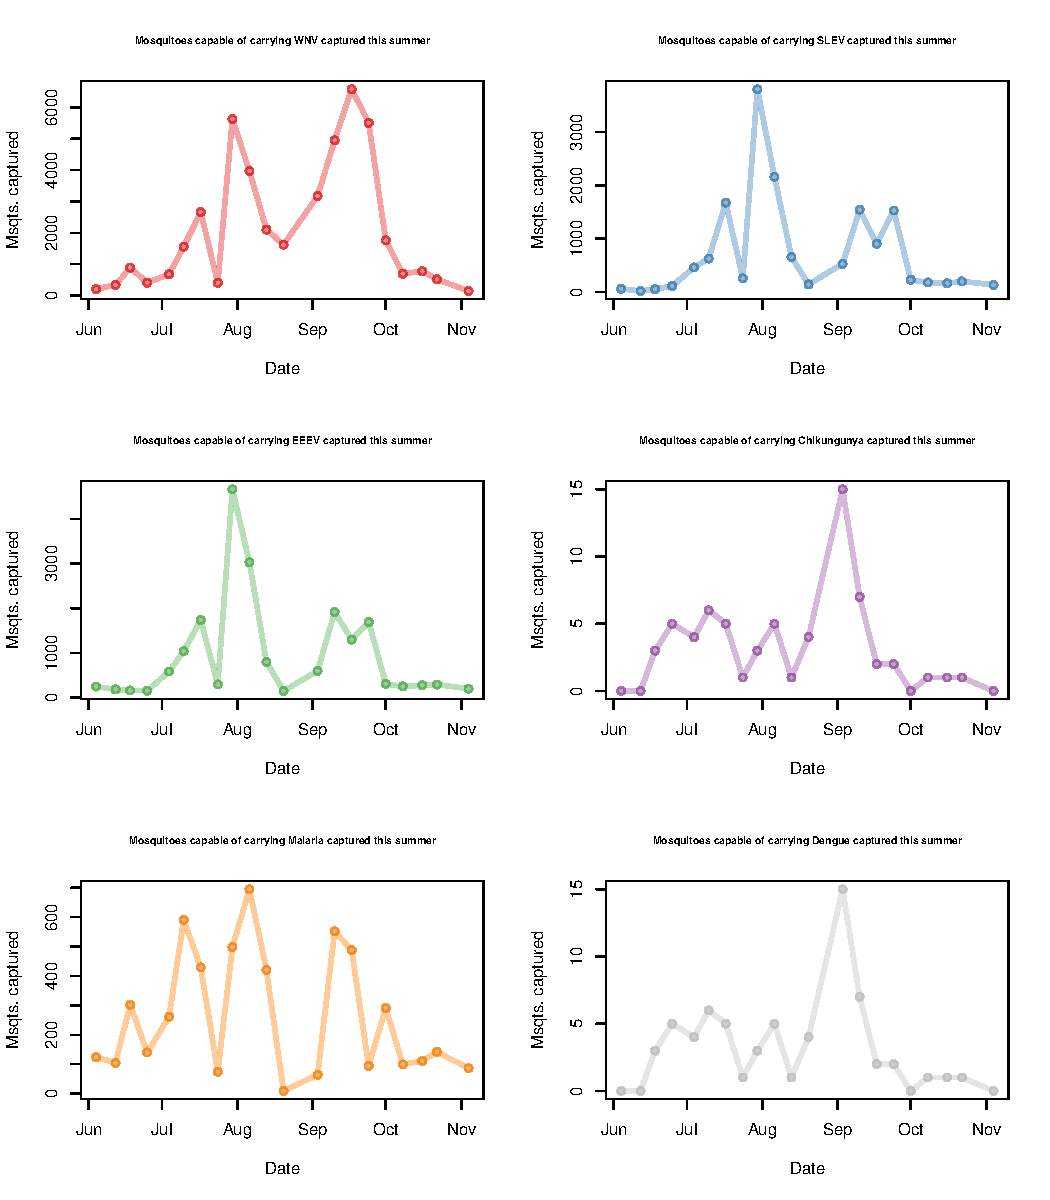
\includegraphics{mosq04nov13-005}
\end{center}
\newpage
\begin{center}
\section*{Trap Site Overview}
\addcontentsline{toc}{section}{Trap Site Overview}

\end{center}

All 10 trap sites are at low levels.
\begin{center}
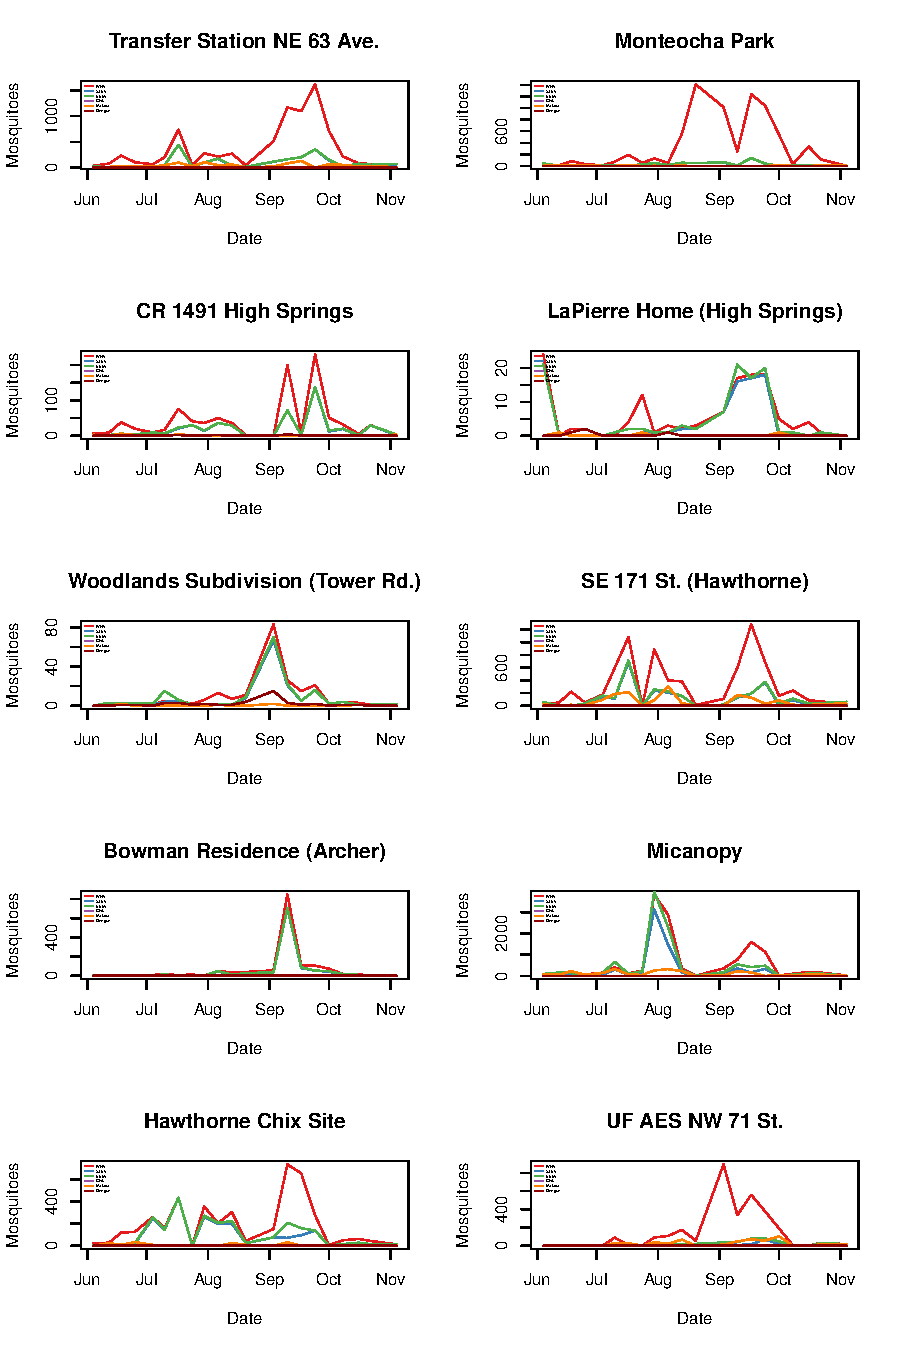
\includegraphics{mosq04nov13-006}
\end{center}
\newpage

\begin{center}
\section*{Trap Site Maps}
\addcontentsline{toc}{section}{Trap Site Maps}

\end{center}

Unlike in Septmeber (which saw particularly high levels in the North part of the county), recent trappings do not suggest abnormal geogrpahical spikes.

\begin{center}
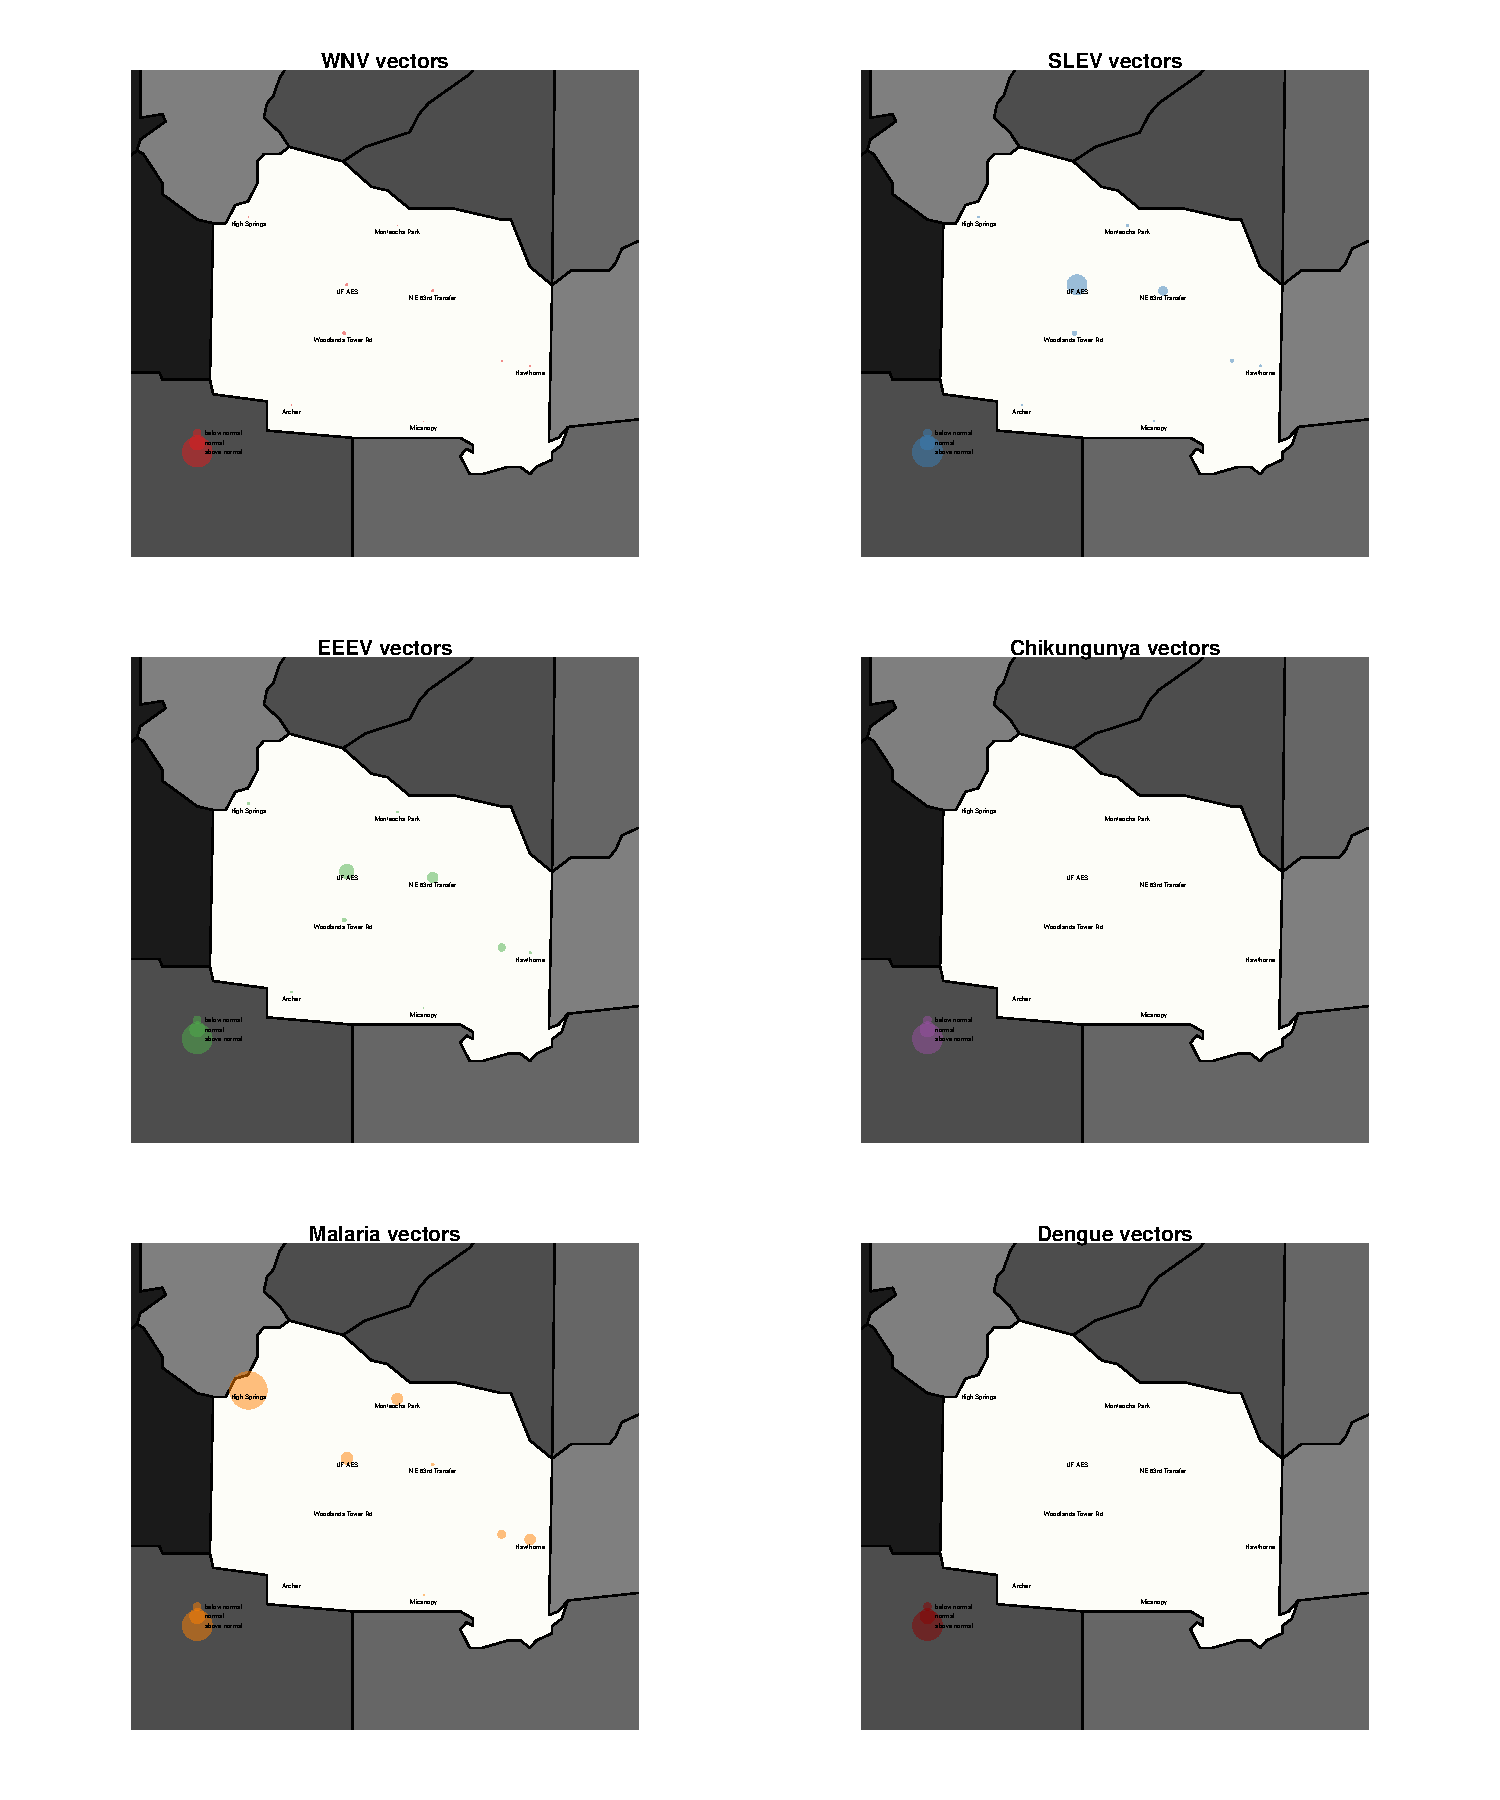
\includegraphics{mosq04nov13-007}
\end{center}
\newpage

\begin{center}
\section*{Disease Type by Trap Site}
\addcontentsline{toc}{section}{Disease Type by Trap Site}

\subsection*{West Nile Virus}
\addcontentsline{toc}{subsection}{West Nile Virus}

\end{center}

Vectors capable of carrying WNV remain low at all sites.\\

\begin{center}
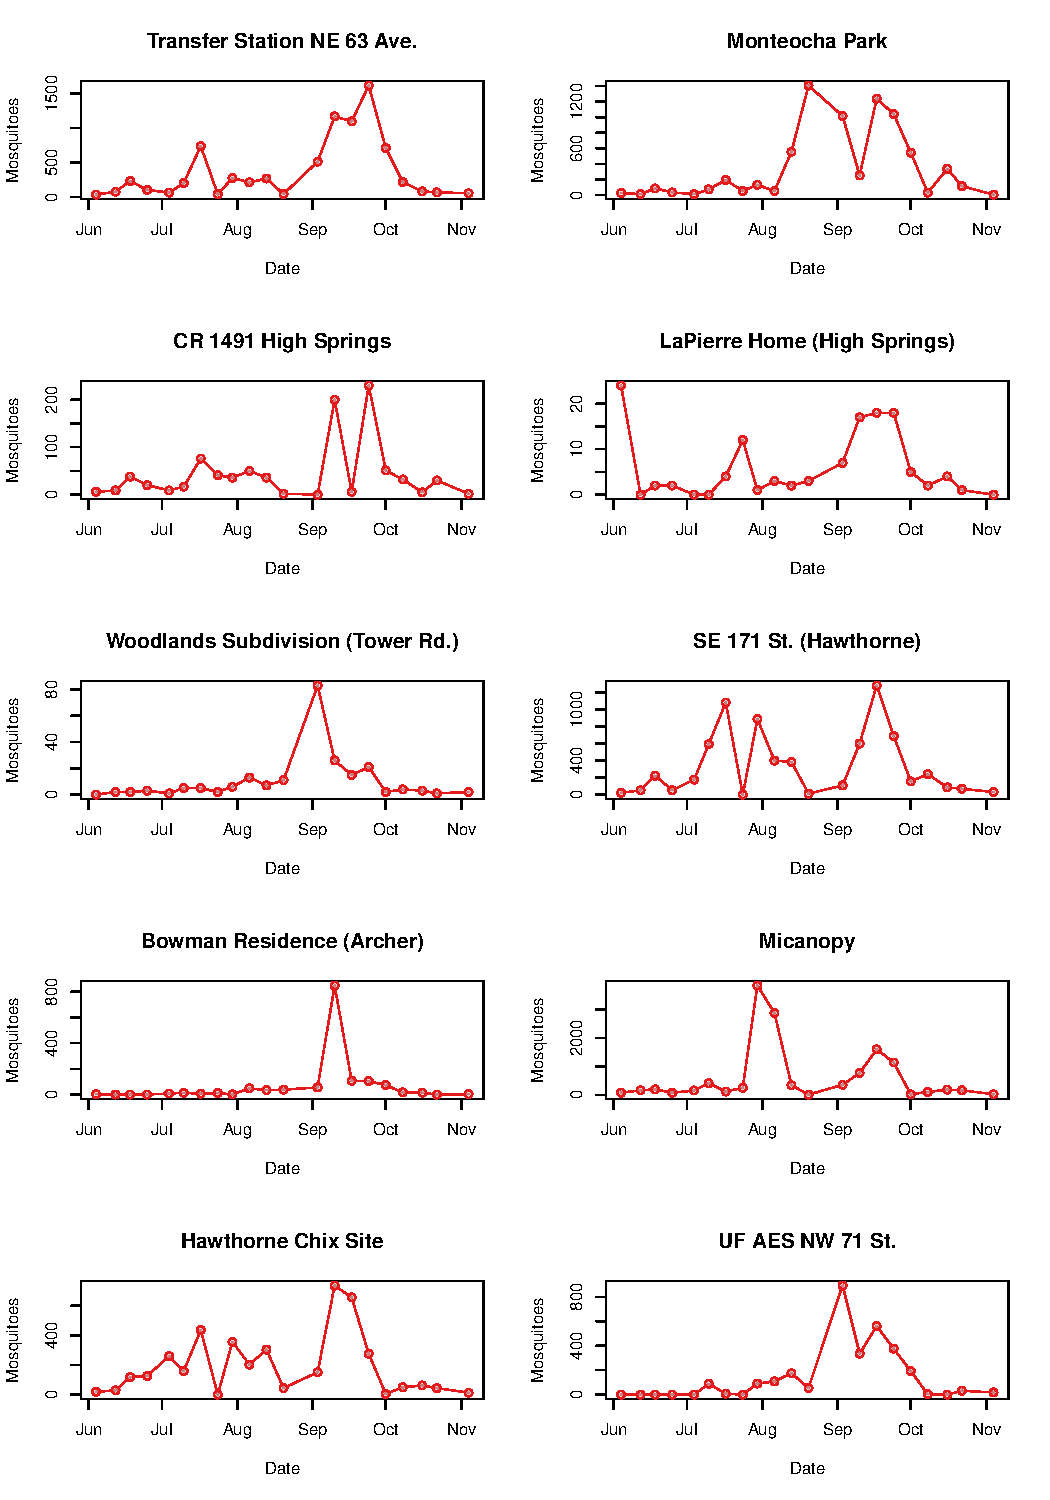
\includegraphics{mosq04nov13-008}
\newpage
\subsection*{SLEV}
\addcontentsline{toc}{subsection}{St. Louis Encephalitis Virus}

\end{center}

Vectors capable of carrying SLEV remain low at all sites.\\

\begin{center}
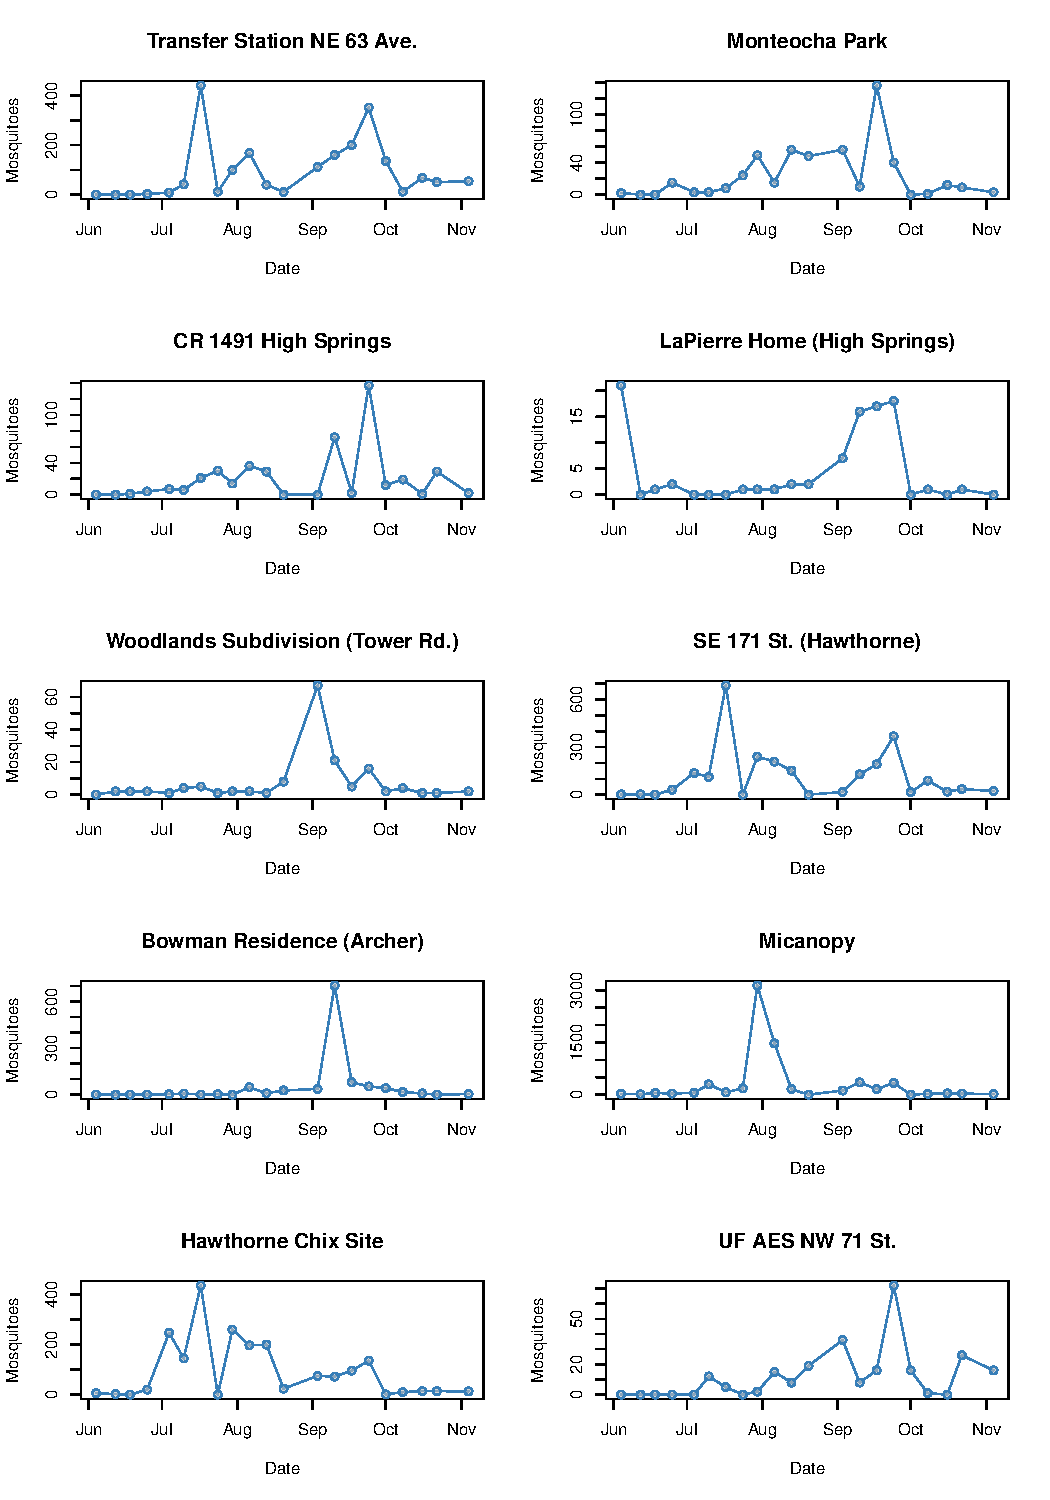
\includegraphics{mosq04nov13-009}

\newpage
\subsection*{EEEV}
\addcontentsline{toc}{subsection}{Eastern Equine Encephalitis Virus}

\end{center}

Vectors capable of carrying EEEV remain low at all sites.\\

\begin{center}
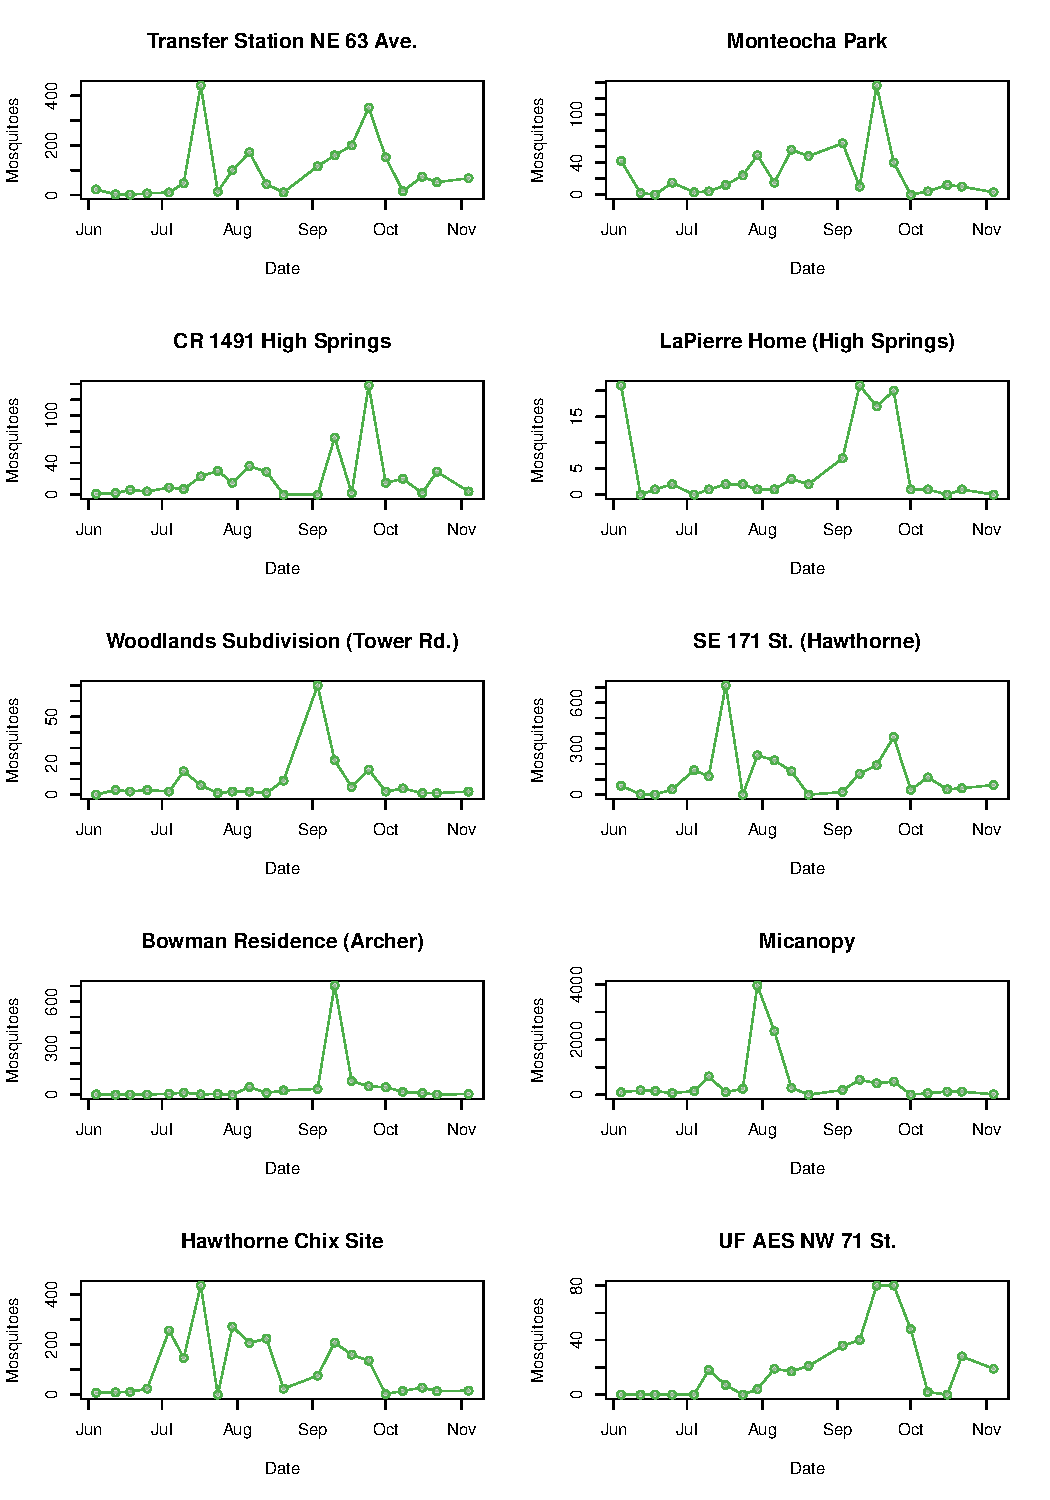
\includegraphics{mosq04nov13-010}
\newpage
\subsection*{Chikungunya}
\addcontentsline{toc}{subsection}{Chikungunya}

\end{center}

Vectors capable of carrying Chikungunya remain low at all sites.\\

\begin{center}
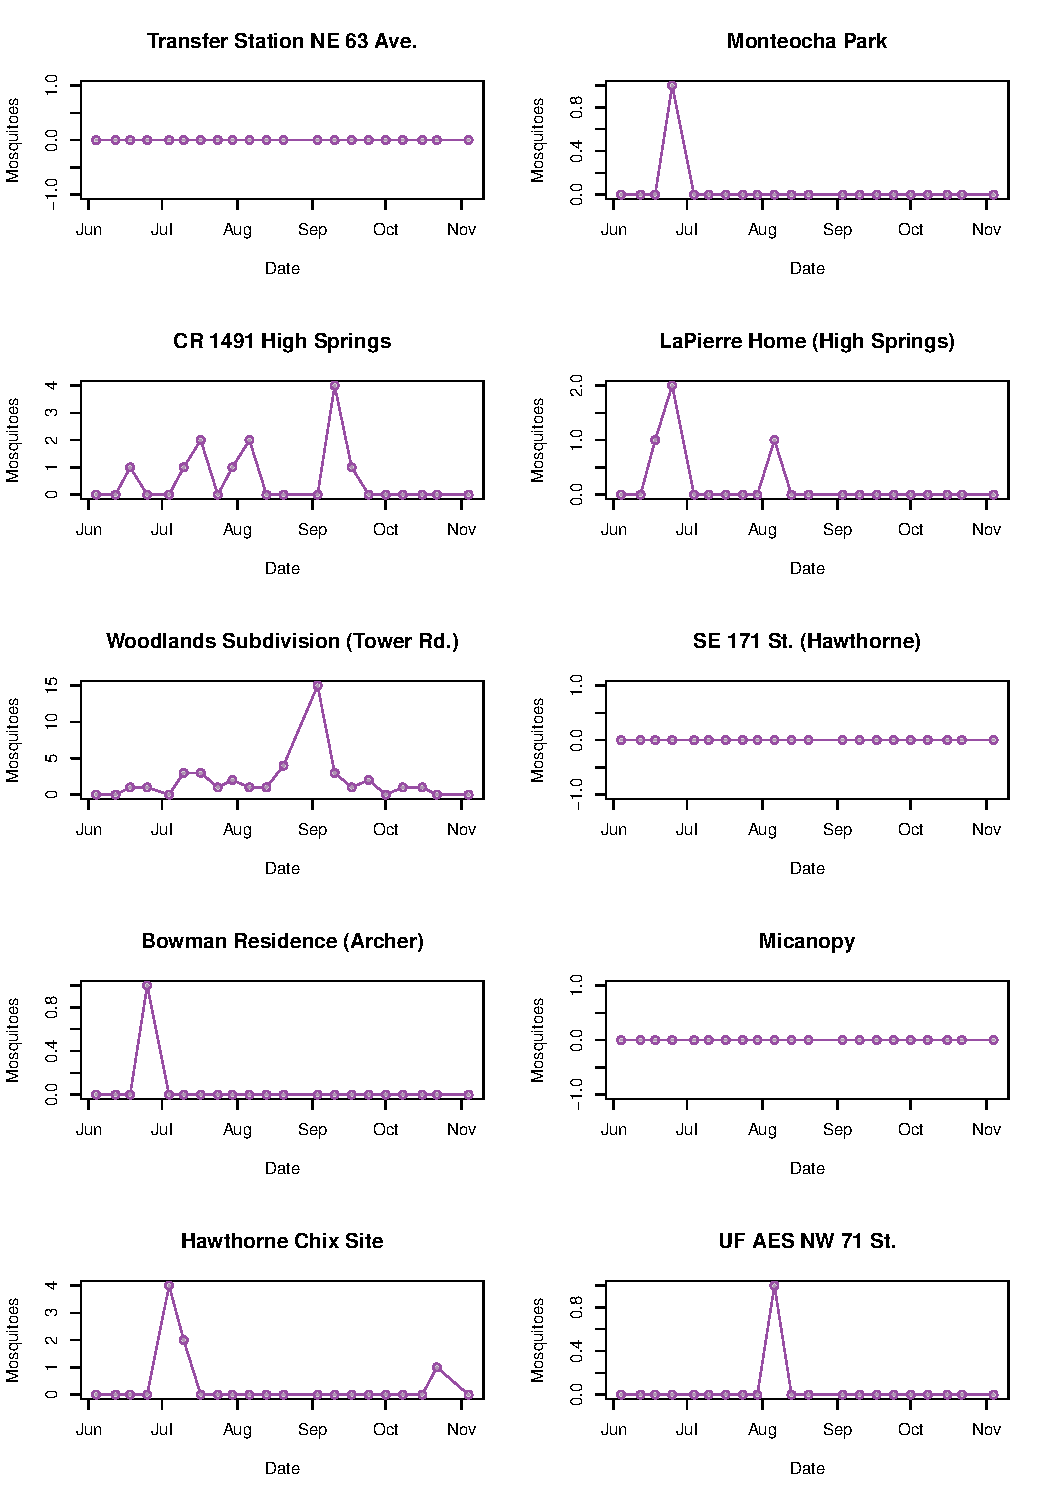
\includegraphics{mosq04nov13-011}
\newpage
\subsection*{Malaria}
\addcontentsline{toc}{subsection}{Malaria}

\end{center}

Vectors capable of carrying Malaria remain low at all sites.\\

\begin{center}
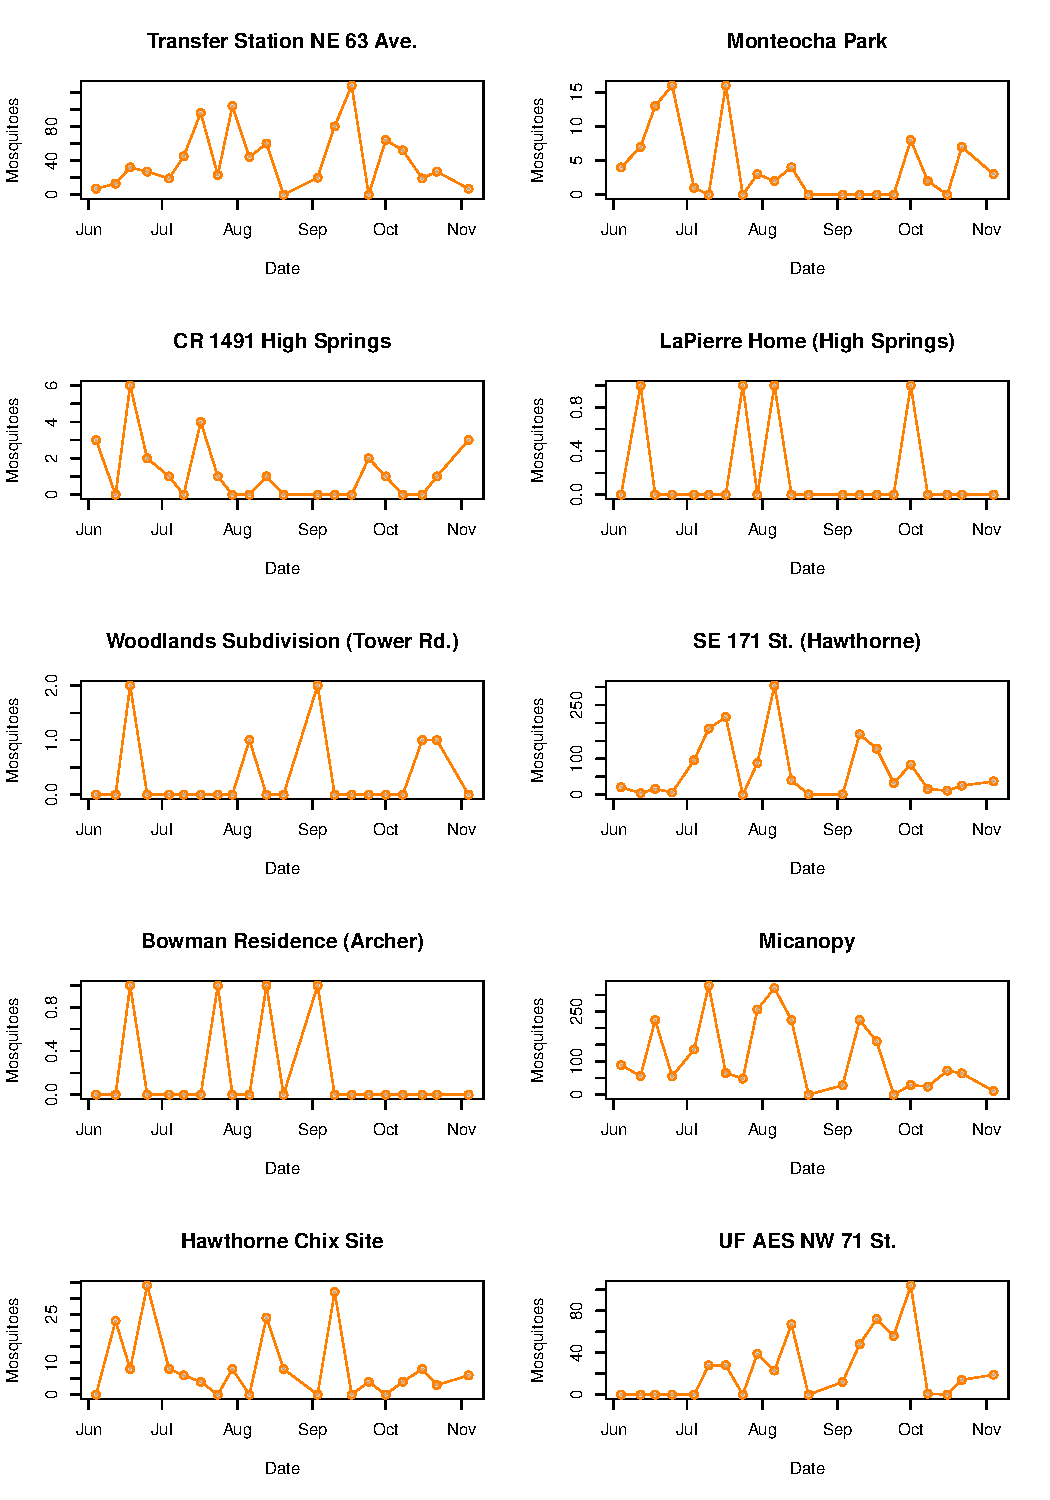
\includegraphics{mosq04nov13-012}
\newpage
\subsection*{Dengue}
\addcontentsline{toc}{subsection}{Dengue}

\end{center}

Vectors capable of carrying Dengue remain low at all sites.\\

\begin{center}
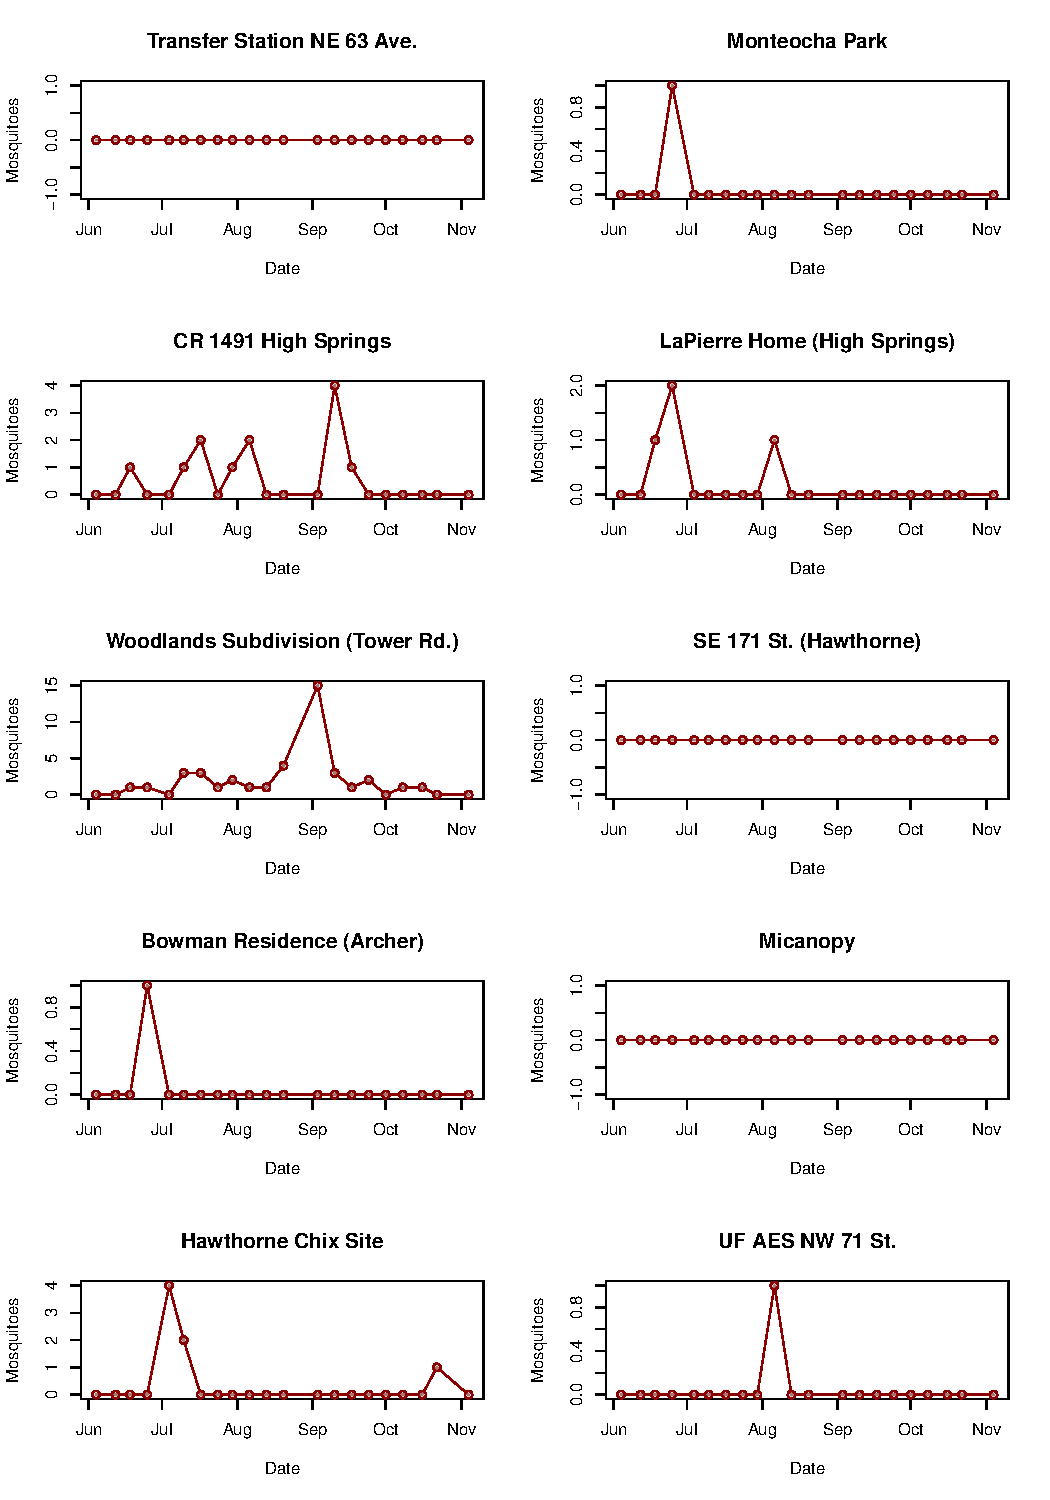
\includegraphics{mosq04nov13-013}

\end{center}
\end{document}
